% Title: glps_renderer figure
% Creator: GL2PS 1.3.8, (C) 1999-2012 C. Geuzaine
% For: Octave
% CreationDate: Fri Dec  6 16:08:22 2019
\setlength{\unitlength}{1pt}
\begin{picture}(0,0)
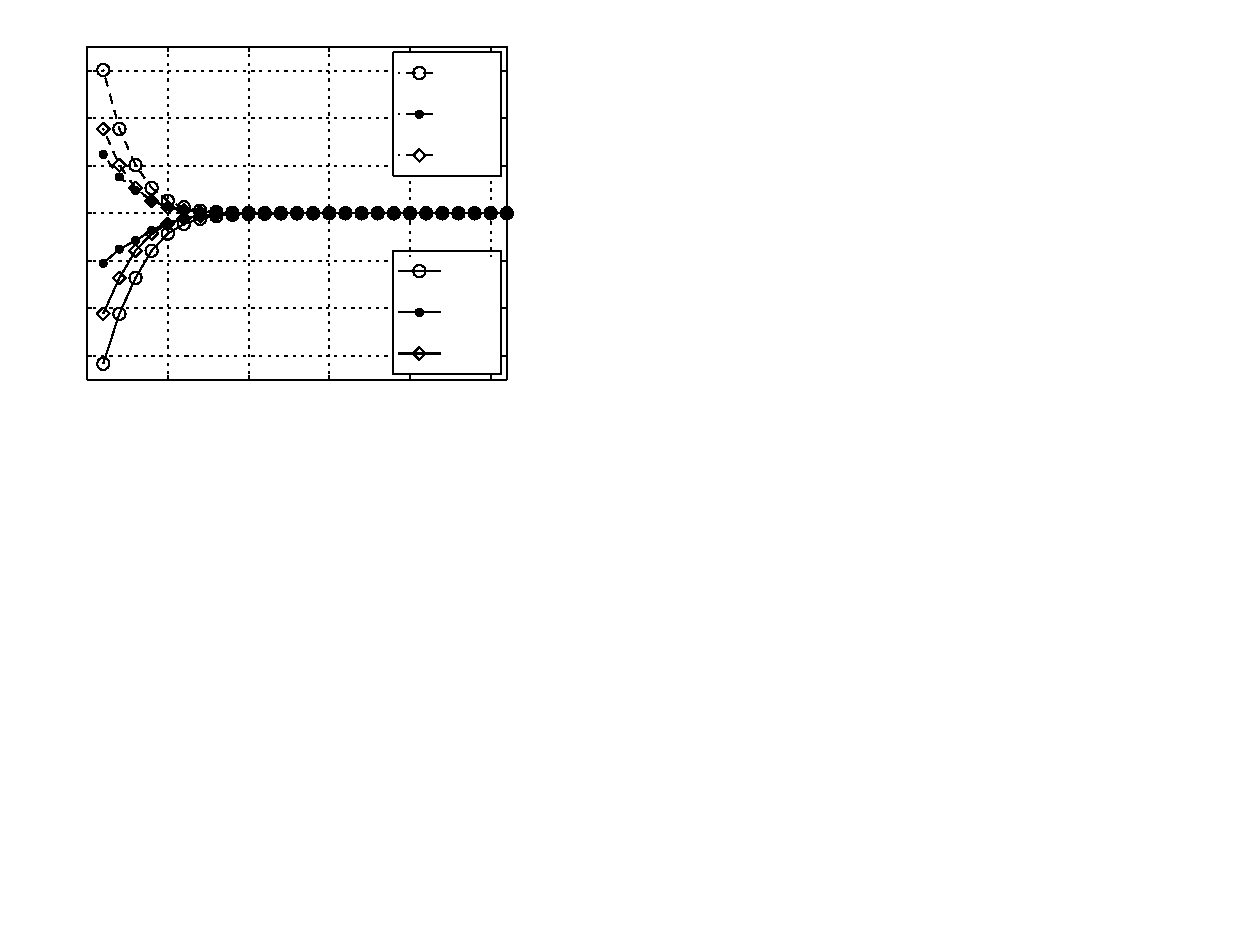
\includegraphics{./figures/under_the_bonnet/perfect/data_perfect}
\end{picture}%
\begin{picture}(576,433)(0,0)
\fontsize{10}{0}
\selectfont\put(33.7998,253.568){\makebox(0,0)[t]{\textcolor[rgb]{0,0,0}{{$0$}}}}
\fontsize{10}{0}
\selectfont\put(72.5498,253.568){\makebox(0,0)[t]{\textcolor[rgb]{0,0,0}{{$5$}}}}
\fontsize{10}{0}
\selectfont\put(111.3,253.568){\makebox(0,0)[t]{\textcolor[rgb]{0,0,0}{{$10$}}}}
\fontsize{10}{0}
\selectfont\put(150.05,253.568){\makebox(0,0)[t]{\textcolor[rgb]{0,0,0}{{$15$}}}}
\fontsize{10}{0}
\selectfont\put(188.8,253.568){\makebox(0,0)[t]{\textcolor[rgb]{0,0,0}{{$20$}}}}
\fontsize{10}{0}
\selectfont\put(227.55,253.568){\makebox(0,0)[t]{\textcolor[rgb]{0,0,0}{{$25$}}}}
\fontsize{10}{0}
\selectfont\put(28.8125,269.97){\makebox(0,0)[r]{\textcolor[rgb]{0,0,0}{{$-3.0$}}}}
\fontsize{10}{0}
\selectfont\put(28.8125,292.79){\makebox(0,0)[r]{\textcolor[rgb]{0,0,0}{{$-2.0$}}}}
\fontsize{10}{0}
\selectfont\put(28.8125,315.61){\makebox(0,0)[r]{\textcolor[rgb]{0,0,0}{{$-1.0$}}}}
\fontsize{10}{0}
\selectfont\put(28.8125,338.43){\makebox(0,0)[r]{\textcolor[rgb]{0,0,0}{{$0.0$}}}}
\fontsize{10}{0}
\selectfont\put(28.8125,361.25){\makebox(0,0)[r]{\textcolor[rgb]{0,0,0}{{$1.0$}}}}
\fontsize{10}{0}
\selectfont\put(28.8125,384.07){\makebox(0,0)[r]{\textcolor[rgb]{0,0,0}{{$2.0$}}}}
\fontsize{10}{0}
\selectfont\put(28.8125,406.89){\makebox(0,0)[r]{\textcolor[rgb]{0,0,0}{{$3.0$}}}}
\fontsize{10}{0}
\selectfont\put(205.969,310.655){\makebox(0,0)[l]{\textcolor[rgb]{0,0,0}{{$\ \ e_x$}}}}
\fontsize{10}{0}
\selectfont\put(205.969,290.889){\makebox(0,0)[l]{\textcolor[rgb]{0,0,0}{{$\ \ u_x$}}}}
\fontsize{10}{0}
\selectfont\put(205.969,271.123){\makebox(0,0)[l]{\textcolor[rgb]{0,0,0}{{$\ \ \delta_x$}}}}
\fontsize{10}{0}
\selectfont\put(205.969,405.738){\makebox(0,0)[l]{\textcolor[rgb]{0,0,0}{{$\ \ e_y$}}}}
\fontsize{10}{0}
\selectfont\put(205.969,385.971){\makebox(0,0)[l]{\textcolor[rgb]{0,0,0}{{$\ \ u_y$}}}}
\fontsize{10}{0}
\selectfont\put(205.969,366.205){\makebox(0,0)[l]{\textcolor[rgb]{0,0,0}{{$\ \ \delta_y$}}}}
\fontsize{10}{0}
\selectfont\put(0,340){\rotatebox{90}{\makebox(0,0){\strut{}Magnitude [m]}}}%
\fontsize{10}{0}
\selectfont\put(133,234){\makebox(0,0){\strut{}Iteration $k$}}%
\end{picture}
